\documentclass[12pt, letterpaper]{article}
%\usepackage{draftwatermark}
%\SetWatermarkText{Copyright \copyright\ 2025\\ Ji, Yonghyeon}
%\SetWatermarkScale{.5}
%\SetWatermarkColor[gray]{0.9}
% --- PACKAGES ---
\usepackage[utf8]{inputenc}
\usepackage[T1]{fontenc}
\usepackage{mathpazo} % Palatino font
\usepackage[margin=.85in]{geometry}
\usepackage{amsmath, amssymb, amsfonts, amsthm, commath}
\usepackage{esint} % For closed integral symbols
\usepackage{fancyhdr} 
\usepackage{xcolor}
\usepackage{tikz} 
\usetikzlibrary{arrows.meta,calc,decorations.markings,patterns,positioning}
\usepackage[most]{tcolorbox} 
\usepackage{booktabs}
\usepackage{tabularx}
\usepackage{hyperref}

% --- MACROS FROM YOUR NOTES ---
\newcommand{\R}{\mathbb{R}}
\newcommand{\C}{\mathbb{C}}
\renewcommand{\d}{\mathrm{d}} % Differential d
\newcommand{\curl}{\mathrm{curl}\,}
\newcommand{\diver}{\mathrm{div}\,}
\renewcommand{\vec}[1]{\mathbf{#1}}
\renewcommand{\d}{\mathrm{d}}
\newcommand{\sol}{\normalfont\bfseries\color{magenta}Sol}
\newcommand{\pderiv}[2]{\frac{\partial #1}{\partial #2}}
\newcommand{\spderiv}[3]{\frac{\partial^2 #1}{\partial #2\partial #3}}

\newtheorem{theorem}{Theorem}[section]
\newtheorem{lemma}[theorem]{Lemma}
\newtheorem{definition}[theorem]{Definition}
\newtheorem{corollary}[theorem]{Corollary}
\theoremstyle{definition}
\newtheorem{example}{Example}

\theoremstyle{remark}
\newtheorem*{remark}{Remark}

% --- COLORS & STYLE ---
\definecolor{themecolor}{RGB}{0, 102, 102} % Teal/Dark Cyan (Vector Calc Theme)
\definecolor{gridcolor}{RGB}{220, 220, 220} 

% --- PAGE HEADER/FOOTER ---
\pagestyle{fancy}
\fancyhf{}
\fancyhead[L]{\small \textsc{Riemann Surfaces and Algebraic Curves}}
\fancyhead[R]{\small Part I --- Multivariable Calculus}
%\fancyfoot[C]{\small Copyright \copyright\ 2025 Ji, Yonghyeon. All rights reserved.}
%\fancyfoot[R]{\thepage}

\fancyfoot[L]{\footnotesize Copyright \copyright\ 2025 Ji, Yonghyeon}
%\fancyfoot[C]{\footnotesize \textit{Part I --- Multivariable Calculus}}
\fancyfoot[R]{\thepage}
\renewcommand{\headrulewidth}{0.4pt}
\renewcommand{\footrulewidth}{0.4pt}

% --- PROBLEM COMMAND ---
\newcounter{probcount}
\newcommand{\makequestion}[2]{
	\clearpage
	\stepcounter{probcount}
	
	% Problem Box
	\begin{tcolorbox}[
		enhanced,
		colback=white,
		colframe=themecolor,
		coltitle=white,
		fonttitle=\bfseries,
		title={Problem \theprobcount: #1},
		sharp corners=south,
		drop fuzzy shadow,
		boxrule=0.5mm,
		top=6mm, bottom=6mm
		]
		%\large 
		#2
	\end{tcolorbox}
	
	% Workspace
	\vfill
	\begin{center}
		\begin{tikzpicture}
			\draw[step=0.5cm,gridcolor,very thin, dash pattern=on 0.5pt off 1.5pt] (0,0) grid (16,15);
		\end{tikzpicture}
	\end{center}
	\vfill
}

% --- TITLE PAGE SETUP ---
\title{
	\vspace{2cm}
	\begin{tcolorbox}[colback=themecolor, colframe=themecolor, sharp corners]
		\centering \color{white}
		\Huge \textbf{Riemann Surfaces and Algebraic Curves}\\
		\vspace{0.5em}
		\Large \textit{A Framework for Understanding Elliptic Curves}
	\end{tcolorbox}
	\Large \textbf{Part I --- Multivariable Calculus}
}
\author{\textbf{Ji, Yonghyeon}}
\date{\today}
\usepackage{pdfpages}
% --- DOCUMENT START ---
\begin{document}

% --- 2. Insert the Cover PDF ---
% 'pages=-' means include all pages (usually just 1 for a cover)
% 'fitpaper=true' adjusts the document page size to match the cover PDF size exactly
\includepdf[pages=-, fitpaper=true]{tikzs/cover-image.pdf}

% --- 3. (Optional) Empty page after cover ---
% If printing double-sided, the back of the cover is usually blank
\cleardoublepage

\newpage	
	
		
% 1. COVER PAGE
\begin{titlepage}
	\centering
	\maketitle
	\thispagestyle{empty}
	
%	\vspace{1cm}
	
	\begin{center}
		\includegraphics[scale=1]{tikzs/generalized_stokes_on_crs.pdf}
	\end{center}
	
	\vfill
	\begin{center}
		\large\bfseries {\scshape WINTER 2026}
	\end{center}
\end{titlepage}

\newpage
%\section*{Preface}
% Summary table + slogans for the FTC hierarchy (LaTeX-ready)
% Requires: \usepackage{booktabs,tabularx,amsmath,amssymb}
% Optional (nice): \usepackage{array} for better column control

\subsection*{The FTC hierarchy}
\begin{table}[ht]
	\centering
	\renewcommand{\arraystretch}{2}
	\setlength{\tabcolsep}{6pt}
	\begin{tabularx}{\linewidth}{
			@{}>{\raggedright\arraybackslash}p{8cm}
%			>{\raggedright\arraybackslash}X
%			>{\raggedright\arraybackslash}p{3.1cm}
%			>{\raggedright\arraybackslash}p{2.6cm}
%			>{\raggedright\arraybackslash}p{2.6cm}
			>{\raggedright\arraybackslash}X@{}
		}
		\toprule
		\textbf{Name} &
		\textbf{Formula} \\ %&
%		\textbf{Interior} &
%		\textbf{Boundary} \\ %&
%		\textbf{Operator} \\
%		\textbf{Slogan} \\
		\midrule
		
		FTC I (Accumulation) &
		$\displaystyle \frac{\d}{\d x}\left(\int_a^x f(t)\,\d t\right)=f(x).$ \\
%		If $F(x)=\displaystyle\int_a^x f(t)\,dt$, then $F'(x)=f(x)$. \\ %&
%		$[a,x]$ &
%		Endpoint $x$ (with basepoint $a$) \\ %&
%%		$\dfrac{d}{dx}$ \\ %&
%		%\textit{Accumulation differentiates to the integrand.} \\
		
		FTC II (Evaluation) &
		$\displaystyle\int_a^b f'(x)\,\d x=f(b)-f(a)$. \\ %&
%		$[a,b]$ &
%		$\{a,b\}$ \\ %&
%%		$\dfrac{d}{dx}$ \\ %&
%%		\textit{Integrate a derivative: get endpoint change.} \\
		
		Fundamental Theorem of Line Integrals &
		$\displaystyle\int_C \nabla\phi\cdot \d\mathbf r=\phi(B)-\phi(A)$. \\ %&
%		Curve $C$ &
%		Endpoints $A,B$ \\ %&
%%		$\nabla$ \\ %&
%%		\textit{Conservative work depends only on endpoints.} \\
		
		Green's Theorem &
		$\displaystyle\oint_{\partial R} P\,\d x+Q\,\d y
		=\iint_R\!\left(\frac{\partial Q}{\partial x}-\frac{\partial P}{\partial y}\right)\,\d A$. \\ %&
%		Region $R\subset\mathbb R^2$ &
%		Simple closed curve $\partial R$ \\ %&
%%		$\operatorname{curl}_{2D}=\frac{\partial Q}{\partial x}-\frac{\partial P}{\partial y}$ \\ %&
%%		\textit{Circulation on the boundary equals curl over the interior.} \\
		
		Stokes' Theorem (3D) &
		$\displaystyle\oint_{\partial S}\mathbf F\cdot \d\mathbf r
		=\iint_S (\nabla\times \mathbf F)\cdot \mathbf n\,\d S$. \\ %&
%		Oriented surface $S\subset\mathbb R^3$ &
%		Boundary curve $\partial S$ \\ %&
%%		$\nabla\times$ \\ %&
%%		\textit{Boundary circulation equals curl through the surface.} \\
		
		Divergence Theorem &
		$\displaystyle\iint_{\partial V}\mathbf F\cdot \mathbf n\,\d S
		=\iiint_V (\nabla\cdot \mathbf F)\,\d V$. \\ %&
%		Volume $V\subset\mathbb R^3$ &
%		Closed surface $\partial V$ \\ %&
%%		$\nabla\cdot$ &
%%		\textit{Flux through the boundary equals divergence in the volume.} \\
		
		Generalized Stokes&
		$\displaystyle \int_{\partial\Omega}\omega=\int_{\Omega} \d \omega$. \\ %&
%		Oriented $k$-manifold $\Omega$ &
%		$(k-1)$-manifold $\partial\Omega$ \\ %&
%%		$d$ (exterior derivative) &
%%		\textit{The boundary integral is the integral of the derivative.} \\
		\bottomrule
	\end{tabularx}
%	\caption{The FTC hierarchy
%		%: interior--boundary correspondences.
%	}
\end{table}

%% --- Optional: slogans-only block (cover-friendly) ---
%\begin{itemize}
%	\item \textbf{FTC I:} Accumulation differentiates to the integrand.
%	\item \textbf{FTC II:} Integrate a derivative: get endpoint change.
%	\item \textbf{Line Integrals:} Conservative work depends only on endpoints.
%	\item \textbf{Green:} Circulation on the boundary equals curl over the interior.
%	\item \textbf{Stokes:} Boundary circulation equals curl through the surface.
%	\item \textbf{Divergence:} Flux through the boundary equals divergence in the volume.
%	\item \textbf{Generalized Stokes:} The boundary integral is the integral of the derivative.
%\end{itemize}

\vfill
\subsection*{Copyright}
\noindent Copyright \copyright\ 2025 by Ji, Yonghyeon All rights reserved. 

No part of this publication may be reproduced, distributed, or transmitted in any form or by any means, including photocopying, recording, or other electronic or mechanical methods, without the prior written permission of the publisher, except in the case of brief quotations embodied in critical reviews and certain other noncommercial uses permitted by copyright law. \\

\medskip

\subsection*{Changelog}
%\large
\begin{tabularx}{\textwidth}{@{} llX @{}} % Column widths specified here, change as needed for your content
	\toprule
	v1.0 & 2025-12-29 & Initial release. \\
	%	v1.1 & 20XX-02-27 & Pellentesque iaculis odio vel nisl ullamcorper, nec faucibus ipsum molestie.\\
	%	v1.2 & 20XX-03-15 & Sed dictum nisl non aliquet porttitor.\\
	\bottomrule
\end{tabularx}

\newpage
\tableofcontents

% 2. PROBLEMS
\newpage
\section{Fundamental Theorem of Calculus}
\begin{tcolorbox}[
	enhanced,colback=white,
	colframe=themecolor,coltitle=white,
	fonttitle=\bfseries,
	title={Fundamental Theorem for Gradient Fields},
	sharp corners=south, drop fuzzy shadow,
	boxrule=0.5mm, top=6mm, bottom=6mm
	]
	If $\vec{F}=\nabla f$ is a conservative vector field and $C$ is a smooth curve from $A$ to $B$, then
	\[ \int_{C}\vec{F}\cdot \d\vec{r}=f(B)-f(A). \]
\end{tcolorbox}
\vfill
\begin{tcolorbox}[
	enhanced,colback=white,
	colframe=themecolor,coltitle=white,
	fonttitle=\bfseries,
	title={Green's Theorem},
	sharp corners=south, drop fuzzy shadow,
	boxrule=0.5mm, top=6mm, bottom=6mm
	]
	For a positively oriented, simple closed curve $C$ bounding a region $R$ in the plane,
	\[ \oint_{C}P~\d x+Q~\d y=\iint_{R}\left(\frac{\partial Q}{\partial x}-\frac{\partial P}{\partial y}\right)\d A. \]
\end{tcolorbox}
\vfill
\begin{tcolorbox}[
	enhanced,colback=white,
	colframe=themecolor,coltitle=white,
	fonttitle=\bfseries,
	title={Divergence Theorem},
	sharp corners=south, drop fuzzy shadow,
	boxrule=0.5mm, top=6mm, bottom=6mm
	]
	Let $\vec{F}$ be a vector field defined on a region $E$ with closed boundary surface $S$ (outward-oriented). Then
	\[ \iiint_{E}\nabla\cdot\vec{F}\; \d V=\iint_{S}\vec{F}\cdot\vec{n}\; \d S. \]
\end{tcolorbox}
\vfill
\begin{tcolorbox}[
	enhanced,colback=white,
	colframe=themecolor,coltitle=white,
	fonttitle=\bfseries,
	title={Stokes' Theorem},
	sharp corners=south, drop fuzzy shadow,
	boxrule=0.5mm, top=6mm, bottom=6mm
	]
	Let $S$ be an oriented surface with boundary curve $C$, and let $\vec{F}$ be a vector field. Then
	\[ \oint_{C}\vec{F}\cdot\d\vec{r}=\iint_{S}(\nabla\times\vec{F})\cdot\vec{n}\d\vec{S}. \]
\end{tcolorbox}
\vfill
\begin{tcolorbox}[
enhanced,colback=white,
colframe=themecolor,coltitle=white,
fonttitle=\bfseries,
title={Triple Integral},
sharp corners=south, drop fuzzy shadow,
boxrule=0.5mm, top=6mm, bottom=6mm
]
To integrate a scalar function $f(x,y,z)$ over a region $E$ in $\mathbb{R}^{3},$
\[ \iiint_{E}f(x,y,z)\; \d V. \]
\end{tcolorbox}

\newpage
\subsection{Gradient Vector Fields}
\begin{tcolorbox}[
	enhanced,colback=white,
	colframe=themecolor,coltitle=white,
	fonttitle=\bfseries,
	title={Scalar field},
	sharp corners=south, drop fuzzy shadow,
	boxrule=0.5mm, top=6mm, bottom=6mm
	]
\begin{definition}
	Let $U\subseteq \mathbb{R}^n$ be an open set. A \emph{scalar field} on $U$ is a function
	\[
	\fullfunction{f}{U}{\R}{\vec{x}}{f(\vec{x})}.
	\]
	Equivalently, to each point $\mathbf x\in U$ the scalar field assigns a real number $f(\mathbf x)$.
\end{definition}
\end{tcolorbox}
\begin{example}[Temperature distribution]
	Let $U=\mathbb{R}^2$. Define
	\[
	T(x,y)=20+10e^{-(x^2+y^2)}.
	\]
	Then $T:U\to\mathbb{R}$ is a scalar field. One may interpret $T(x,y)$ as the temperature (in degrees) at the point $(x,y)$.
	Notice that $T(0,0)=30$ and $T(x,y)\to 20$ as $x^2+y^2\to\infty$, so the temperature is highest at the origin and decays outward.
	
	\medskip
	
\begin{center}
\includegraphics[scale=1]{tikzs/examples/temp_dist.pdf}
\end{center}

\end{example}


\begin{tcolorbox}[
	enhanced,colback=white,
	colframe=themecolor,coltitle=white,
	fonttitle=\bfseries,
	title={Vector field},
	sharp corners=south, drop fuzzy shadow,
	boxrule=0.5mm, top=6mm, bottom=6mm
	]
\begin{definition}
	Let $U\subseteq \mathbb{R}^n$ be an open set. A \emph{vector field} on $U$ is a function
	\[
	\fullfunction{\vec{F}}{U}{\R^n}{\vec{x}}{\vec{F}(\vec{x})}.
	\]
	Equivalently, to each point $\mathbf x\in U$ the vector field assigns a vector $\mathbf F(\mathbf x)\in \mathbb{R}^n$.
	In coordinates, one often writes
	\[
	\mathbf F(\mathbf x)=\langle F_1(\mathbf x),F_2(\mathbf x),\dots,F_n(\mathbf x)\rangle,
	\]
	where each component function $F_i:U\to\mathbb{R}$ is a scalar field on $U$.
\end{definition}
\end{tcolorbox}
\begin{example}[Rotation field]
	Let $U=\mathbb{R}^2$. Define
	\[
	\mathbf F(x,y)=\langle -y,\; x\rangle.
	\]
	Then $\mathbf F:U\to\mathbb{R}^2$ is a vector field. At each point $(x,y)$ it assigns the vector $(-y,x)$, which is perpendicular to
	$\langle x,y\rangle$ and tangent to the circle $x^2+y^2=\text{constant}$.
	Moreover,
	\[
	\|\mathbf F(x,y)\|=\sqrt{x^2+y^2},
	\]
	so the magnitude increases linearly with the distance from the origin. This field models a rigid counterclockwise rotational flow about the origin.
	
	\medskip
	
	\begin{center}
		\includegraphics[scale=1]{tikzs/examples/rotation_field.pdf}
	\end{center}
\end{example}

%\begin{remark}
%	A vector field $\mathbf F:U\to\mathbb{R}^n$ can be regarded as a matrix-valued function
%	\[
%	\mathbf F:U\to M_{n\times 1}(\mathbb{R}),
%	\qquad
%	\mathbf F(\mathbf x)=
%	\begin{pmatrix}
%		F_1(\mathbf x)\\
%		F_2(\mathbf x)\\
%		\vdots\\
%		F_n(\mathbf x)
%	\end{pmatrix}.
%	\]
%	Thus a vector field is equivalently an $n\times 1$ matrix (column vector) of scalar fields.
%	
%	More generally, a \emph{matrix field} on $U$ is a function
%	\[
%	A:U\to M_{m\times n}(\mathbb{R}),
%	\qquad
%	A(\mathbf x)=\big(a_{ij}(\mathbf x)\big),
%	\]
%	where each entry $a_{ij}:U\to\mathbb{R}$ is a scalar field.
%\end{remark}

\newpage
\begin{remark}
\begin{definition}[Conservative vector field]
	Let $U\subseteq \mathbb{R}^n$ be an open set and let $\vec F:U\to\mathbb{R}^n$ be a vector field.
	We say that $\vec F$ is \emph{conservative} on $U$ if there exists a scalar field $f:U\to\mathbb{R}$ of class $C^{1}$
	such that
	\[
	\vec F=\nabla f \quad \text{on } U.
	\]
	In this case, $f$ is called a \emph{potential function} for $\vec F$.
\end{definition}
\begin{remark}[Equivalent characterization]
	A vector field $\vec F$ on $U$ is conservative if and only if for every piecewise $C^{1}$ curve $C$ in $U$ with endpoints
	$\vec A,\vec B$, the line integral $\int_C \vec F\cdot d\vec r$ depends only on $\vec A$ and $\vec B$ (path independence).
	Equivalently,
	\[
	\oint_C \vec F\cdot d\vec r = 0
	\]
	for every piecewise $C^{1}$ closed curve $C$ in $U$.
\end{remark}

\end{remark}

\begin{definition}[Gradient operator]
	Let $U\subseteq \mathbb{R}^n$ be open. The \emph{gradient operator} (or \emph{nabla operator})
	is the map
	\[
	\nabla: C^{1}(U)\longrightarrow C^{0}(U,\mathbb{R}^n)
	\]
	defined by
	\[
	(\nabla f)(\vec x)=
	\begin{pmatrix}
		\dfrac{\partial f}{\partial x_1}(\vec x)\\[6pt]
		\dfrac{\partial f}{\partial x_2}(\vec x)\\
		\vdots\\
		\dfrac{\partial f}{\partial x_n}(\vec x)
	\end{pmatrix},
	\qquad \vec x=(x_1,\dots,x_n)\in U.
	\]
\end{definition}

\begin{remark}[Directional derivative characterization]
	For $f\in C^{1}(U)$ and $\vec x\in U$, the vector $\nabla f(\vec x)\in\mathbb{R}^n$ is uniquely characterized by the property that
	\[
	D_{\vec v}f(\vec x)=\nabla f(\vec x)\cdot \vec v
	\qquad \text{for all }\vec v\in\mathbb{R}^n,
	\]
	where $D_{\vec v}f(\vec x)$ denotes the directional derivative of $f$ at $\vec x$ in the direction $\vec v$.
\end{remark}

%\begin{proposition}
[Linearity of $\nabla$]
	Let $f,g\in C^{1}(U)$ and $a,b\in\mathbb{R}$. Then
	\[
	\nabla(af+bg)=a\,\nabla f+b\,\nabla g.
	\]
%\end{proposition}

\begin{remark}[Jacobian/transpose viewpoint]
	For $f\in C^{1}(U)$, the total derivative at $\vec x\in U$ is the linear map
	\[
	Df(\vec x):\mathbb{R}^n\to\mathbb{R},
	\qquad
	Df(\vec x)\,\vec v = D_{\vec v}f(\vec x).
	\]
	In coordinates, $Df(\vec x)$ is represented by the $1\times n$ Jacobian row matrix
	\[
	Df(\vec x)=
	\begin{pmatrix}
		\dfrac{\partial f}{\partial x_1}(\vec x) & \cdots & \dfrac{\partial f}{\partial x_n}(\vec x)
	\end{pmatrix},
	\]
	and the gradient is its transpose:
	\[
	\nabla f(\vec x) = \bigl(Df(\vec x)\bigr)^{\mathsf T}.
	\]
	Consequently, for any $\vec v\in\mathbb{R}^n$,
	\[
	D_{\vec v}f(\vec x)=Df(\vec x)\,\vec v = \bigl(\nabla f(\vec x)\bigr)^{\mathsf T}\vec v
	= \nabla f(\vec x)\cdot \vec v.
	\]
\end{remark}


\newpage
\begin{tcolorbox}[
	enhanced,colback=white,
	colframe=themecolor,coltitle=white,
	fonttitle=\bfseries,
	title={Fundamental Theorem for Gradient Fields},
	sharp corners=south, drop fuzzy shadow,
	boxrule=0.5mm, top=6mm, bottom=6mm
	]
	\begin{theorem}
		Let $U\subset \mathbb{R}^n$ be an open set and let $f:U\to \mathbb{R}$ be continuously differentiable ($f\in C^{1}(U)$).
		Let $C$ be a piecewise $C^{1}$ curve in $U$ with a piecewise $C^{1}$ parametrization \[
		\mathbf r:[a,b]\to U.
		\]
		If $\mathbf r(a)=\mathbf A$ and $\mathbf r(b)=\mathbf B$, then
		\[
		\int_{C}\nabla f\cdot d\mathbf r \;=\; f(\mathbf B)-f(\mathbf A).
		\]
		In particular, the line integral of a gradient field depends only on the endpoints of the curve.
	\end{theorem}
\end{tcolorbox}
\begin{proof}
	By definition of the line integral of a vector field along a parametrized curve,
	\[
	\int_{C}\nabla f\cdot d\mathbf r
	\;=\;
	\int_{a}^{b}\nabla f(\mathbf r(t))\cdot \mathbf r'(t)\,dt.
	\]
	Define a scalar-valued function $g:[a,b]\to\mathbb R$ by $g(t)=f(\mathbf r(t))$.
	Since $f\in C^{1}(U)$ and $\mathbf r$ is piecewise $C^{1}$, the composition $g$ is piecewise $C^{1}$.
	On any subinterval where $\mathbf r$ is $C^{1}$, the multivariable chain rule gives
	\[
	g'(t)=\nabla f(\mathbf r(t))\cdot \mathbf r'(t).
	\]
	Hence on each such subinterval we have $\nabla f(\mathbf r(t))\cdot \mathbf r'(t)=g'(t)$, and summing over the finitely many
	smooth pieces yields
	\[
	\int_{a}^{b}\nabla f(\mathbf r(t))\cdot \mathbf r'(t)\,dt
	=
	\int_{a}^{b} g'(t)\,dt.
	\]
	By the (single-variable) Fundamental Theorem of Calculus,
	\[
	\int_{a}^{b} g'(t)\,dt=g(b)-g(a).
	\]
	Substituting back $g(t)=f(\mathbf r(t))$ gives
	\[
	g(b)-g(a)=f(\mathbf r(b))-f(\mathbf r(a))
	=
	f(\mathbf B)-f(\mathbf A).
	\]
	Therefore,
	\[
	\int_{C}\nabla f\cdot d\mathbf r \;=\; f(\mathbf B)-f(\mathbf A),
	\]
	as claimed.
\end{proof}

%\begin{corollary}[Closed Curves]
%	If $C$ is a closed curve (i.e., $\mathbf r(a)=\mathbf r(b)$), then
%	\[
%	\oint_{C}\nabla f\cdot d\mathbf r = 0.
%	\]
%\end{corollary}

\newpage\noindent
Consider a small rectangle centered at \((x_0,y_0)\) with side lengths \(\Delta x,\Delta y\). 
\begin{figure}[h!]
	\centering
	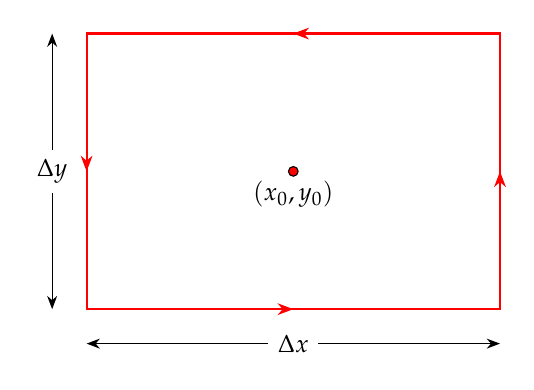
\begin{tikzpicture}[scale=1.75, font=\small, >=Stealth]
		% Draw rectangle and center point
		\draw[thick, red] (-1.5,-1) rectangle (1.5,1);
		\draw[fill=red] (0,0) circle (1pt) node[below] {$(x_0, y_0)$};
		% Add arrows for CCW circulation path
		\draw[-{Stealth[length=2mm]}, red] (-1.5, -1) -- (0, -1);
		\draw[-{Stealth[length=2mm]}, red] (1.5, -1) -- (1.5, 0);
		\draw[-{Stealth[length=2mm]}, red] (1.5, 1) -- (0, 1);
		\draw[-{Stealth[length=2mm]}, red] (-1.5, 1) -- (-1.5, 0);
		\draw[<->] (0-1.5, 0-1.25) -- ++(3, 0) node[midway, fill=white] {$\Delta x$};
		\draw[<->] (0-1.75, 0-1) -- ++(0, 2) node[midway, fill=white] {$\Delta y$};
		% Label path segments
		%		\node at (0, -1.7) {Bottom: $\int P(x, y_0-\frac{\Delta y}{2}) dx$};
		%		\node at (0, 1.45) {Top: $\int P(x, y_0+\frac{\Delta y}{2}) (-dx)$};
		%		\node[rotate=90] at (1.95, 0) {Right: $\int Q(x_0+\frac{\Delta x}{2}, y) dy$};
		%		\node[rotate=90] at (-2.2, 0) {Left: $\int Q(x_0-\frac{\Delta x}{2}, y) (-dy)$};
		% Illustrate change in P and Q
		%		\draw[->, thick, blue] (0, 1) -- (1.2, 1) node[above] {$P_{top}$};
		%		\draw[->, thick, blue] (0, -1) -- (0.8, -1) node[below] {$P_{bot}$};
		%		\node[red, align=center] at (2.5, 0) {Difference in P\\contributes\\$-P_y \Delta x \Delta y$};
		%		\draw[->, thick, green!50!black] (1.5, 0) -- (1.5, 0.8) node[right] {$Q_{right}$};
		%		\draw[->, thick, green!50!black] (-1.5, 0) -- (-1.5, 1.0) node[left] {$Q_{left}$};
		%		\node[red, align=center] at (-2.5, 0) {Difference in Q\\contributes\\$Q_x \Delta x \Delta y$};
	\end{tikzpicture}
	\caption{Circulation around an infinitesimal rectangle.}
	\label{fig:local_circ}
\end{figure}

\noindent
The total counterclockwise circulation is the sum of the line integrals along the four edges:
\[
\oint_{\partial R}\vec F\cdot \d\vec r
=\int_{\text{bottom}}P\,\d x+\int_{\text{right}}Q\,\d y+\int_{\text{top}}P\,\d x+\int_{\text{left}}Q\,\d y.
\]
We will approximate the value of $P$ or $Q$ along each edge as being constant, equal to its value at the midpoint of that edge. We find this value using a first-order Taylor expansion from the center point $(x_0, y_0)$.

For a simple function of one variable, $f(x)$, if we know its value at a point $a$, then we can estimate its value at a nearly point $a+h$ using the tangent line at $a$: 
\begin{center}
	\begin{minipage}{.49\textwidth}
		\begin{align*}
			f(a+h)&\approx f(a)+f'(a)\cdot h \quad\text{or}\\
			f(x)&\approx f(a)+f'(a)\cdot (x-a).
		\end{align*} 
		
	\end{minipage}
	\begin{minipage}{.49\textwidth}
		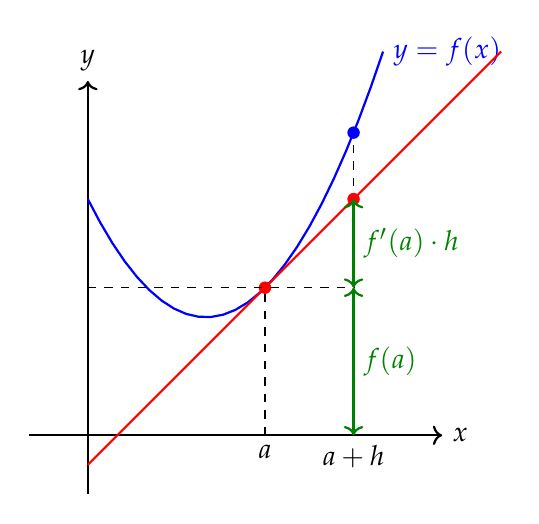
\begin{tikzpicture}[
			scale=1.5,
			declare function={f(\x) = (\x-1)^2 + 1;}
			]
			% Axes
			\draw[->, thick] (-0.5,0) -- (3,0) node[right] {$x$};
			\draw[->, thick] (0,-0.5) -- (0,3) node[above] {$y$};
			% The curve f(x)
			\draw[blue, thick, domain=0:2.5] plot (\x, {f(\x)}) node[right] {$y=f(x)$};
			% Point 'a'
			\def\a{1.5}
			\node[below] at (\a,0) {$a$};
			\draw[dashed] (\a,0) -- (\a, {f(\a)});
			\fill[red] (\a, {f(\a)}) circle (1.5pt);
			% Point 'a+h'
			\def\h{.75}
			\node[below] at (\a+\h,0) {$a+h$};
			\draw[dashed] (\a+\h,0) -- (\a+\h, {f(\a+\h)});
			% Tangent line at 'a'
			% f'(x) = 2(x-1), so f'(a) = 2(a-1)
			\draw[red, thick, domain=0:3.5] plot (\x, {f(\a) + 2*(\a-1)*(\x-\a)});
			% Show f(a)
			\draw[<->, green!50!black, thick] (\a+\h, 0) -- (\a+\h, {f(\a)}) node[midway, right] {$f(a)$};
			% Show the approximation f(a) + f'(a)h
			\pgfmathsetmacro{\approxY}{f(\a) + 2*(\a-1)*\h}
			\fill[red] (\a+\h, \approxY) circle (1.5pt);
			%	\draw[red, dashed] (\a+\h, \approxY) -- (\a+\h, 0);
			
			% Show the actual value f(a+h)
			\fill[blue] (\a+\h, {f(\a+\h)}) circle (1.5pt);
			%	\node[right, blue] at (\a+\h, {f(\a+\h)}) {Actual value: $f(a+h)$};
			%	\node[right, red] at (\a+\h, \approxY) {Approximation: $f(a)+f'(a)h$};
			
			% Label the components of the approximation
			\draw[<->, green!50!black, thick] (\a+\h, {f(\a)}) -- (\a+\h, \approxY) node[midway, right] {$f'(a)\cdot h$};
			\draw[dashed] (0, {f(\a)}) -- (\a+\h, {f(\a)});
		\end{tikzpicture}
	\end{minipage}
\end{center}
In words, ``New Value $\approx$ Old Value + (Rate of Change) $\times$ (Small Step)''. 

\newpage\noindent
For a function of two variables like $P(x,y)$, the idea is identical, but the ``rate of change'' now has two components (one for each direction), and the ``tangent line'' becomes a ``tangent plane''.
The general first-order Taylor expansion for $P(x,y)$ around a center point $(x_0,y_0)$ is
\[
P(x_0+a, y_0+b) \approx P(x_0, y_0) + \pderiv{P}{x}(x_0, y_0) \cdot a + \pderiv{P}{y}(x_0, y_0) \cdot b
\] Here, $a$ is the small step in the $x$-direction, and $b$ is the small step in the $y$-direction.

\paragraph{1. The Horizontal Paths}
These integrals involve the horizontal component of $P(x,y)$.
\begin{itemize}
	\item \textbf{Bottom Path ($\rightarrow$):} 
	\begin{align*}
	&P\left(x, y_0 - \frac{\Delta y}{2}\right) \approx P(x_0,y_0) - \pderiv{P}{y}(x_0,y_0)\frac{\Delta y}{2}\\
	&\implies\int_{\text{bottom}} P\,\d x \approx\int_{-\Delta x/2}^{\Delta x/2}\left(P_0+P_xs-P_y\frac{\Delta y}{2}\right)\; ds\qquad(x=x_0+s,\; dx=ds)\\
	&\implies
	\int_{\text{bottom}} P\,\d x \approx \left( P(x_0,y_0) - \pderiv{P}{y}(x_0,y_0)\frac{\Delta y}{2} \right) (\Delta x)
	\end{align*}
Note that \[
\int_{-\Delta x/2}^{\Delta x/2} P_x s\; ds=P_x\left[\frac{s^2}{2}\right]_{-\Delta x/2}^{\Delta x/2}=P_x\left(\frac{(\Delta x/2)^2}{2}-\frac{(\Delta x/2)^2}{2}\right)=0.
\]
	\item \textbf{Top Path ($\leftarrow$):}
	\[ P\left(x, y_0 + \frac{\Delta y}{2}\right) \approx P(x_0,y_0) + \pderiv{P}{y}\frac{\Delta y}{2}\implies\int_{\text{top}}P\,\d x \approx -\left( P(x_0,y_0) + \pderiv{P}{y}\frac{\Delta y}{2} \right) (\Delta x) \]
\end{itemize} Here, we are left with only the parts that describe the \textit{change} in $P$ with respect to $y$.
\[
\int_{\text{bottom}} P\,\d x + \int_{\text{top}} P\,\d x \approx \left(-\pderiv{P}{y}\frac{\Delta y}{2}\right)\Delta x - \left(\pderiv{P}{y}\frac{\Delta y}{2}\right)\Delta x = -\pderiv{P}{y}\Delta x\Delta y
\]
\paragraph{2. The Vertical Paths}
These integrals involve the vertical component of $Q(x,y)$.
\begin{itemize}
	\item \textbf{Right Path ( $\uparrow$ ):} 
	\[ Q\left(x_0 + \frac{\Delta x}{2}, y\right) \approx Q(x_0,y_0) + \pderiv{Q}{x}\frac{\Delta x}{2}\implies\int_{\text{right}}Q\,\d y \approx \left( Q(x_0,y_0) + \pderiv{Q}{x}\frac{\Delta x}{2} \right) (\Delta y) \]
	\item \textbf{Left Path ( $\downarrow$ ):} 
	\[ Q\left(x_0 - \frac{\Delta x}{2}, y\right) \approx Q(x_0,y_0) - \pderiv{Q}{x}\frac{\Delta x}{2}\implies\int_{\text{left}}Q\,\d y \approx -\left( Q(x_0,y_0) - \pderiv{Q}{x}\frac{\Delta x}{2} \right) (\Delta y) \]
\end{itemize} Here, we are left with only the parts that describe the \textit{change} in $Q$ with respect to $x$.
\[
\int_{\text{right}}Q\,\d y + \int_{\text{left}}Q\,\d y \approx \left(\pderiv{Q}{x}\frac{\Delta x}{2}\right)\Delta y + \left(\pderiv{Q}{x}\frac{\Delta x}{2}\right)\Delta y = \pderiv{Q}{x}\Delta x\Delta y
\]

Now we sum the results from the horizontal and vertical pairs:
\begin{align*}
	\oint_{\partial R}\vec F\cdot d\vec r &\approx \left(-\pderiv{P}{y}\Delta x\Delta y\right) + \left(\pderiv{Q}{x}\Delta x\Delta y\right) \\
	&= \left(\pderiv{Q}{x} - \pderiv{P}{y}\right)\Delta x\Delta y
\end{align*}
This shows that the total circulation around the tiny loop is approximately the quantity $\left(\pderiv{Q}{x} - \pderiv{P}{y}\right)$ multiplied by the area of the loop ($\Delta A = \Delta x \Delta y$).

To get the property \textit{at the point} $(x_0, y_0)$, we find the circulation \textbf{density}. We divide by the area and take the limit as the rectangle shrinks to zero.
\[
\lim_{\Delta A\to 0}\frac{1}{\Delta A}\oint_{\partial R}\vec F\cdot \d\vec r = \pderiv{Q}{x}(x_0, y_0) - \pderiv{P}{y}(x_0, y_0)
\]
This is why we call the scalar quantity $\pderiv{Q}{x} - \pderiv{P}{y}$ the \textbf{curl}: it is the circulation per unit area at a point, which measures the local rotational tendency of the field.

If \(C=\partial D\) is a positively oriented simple closed curve enclosing a region \(D\),
Green's theorem states \[
%\oint_{C}\vec F\cdot\d\vec r
%=\iint_{D}\Big(\frac{\partial Q}{\partial x}-\frac{\partial P}{\partial y}\Big)\,\d A.
\underbrace{\oint_{C}\vec F\cdot\d\vec r}_{\substack{\textbf{Line Integral}\\ \textbf{(Total Circulation)}}}= \underbrace{\iint_{D}\Big(\frac{\partial Q}{\partial x}-\frac{\partial P}{\partial y}\Big)\,\d A}_{\substack{\textbf{Double Integral}\\ \textbf{(Sum of Local Curls)}}}
\]

\newpage
\begin{enumerate}
	\item Let $\vec{F}=\langle 2x, 2y \rangle$. Show that $\vec{F}$ is conservative and compute \[
	\int_{C}\vec{F}\cdot\d\vec{r}
	\] where $C$ is any path from $(0,0)$ to $(1, 1)$.
%	\begin{center}
%	\includegraphics[scale=1]{tikzs/1-1.pdf}
%	\end{center}
\begin{proof}[\sol]
Let $\vec F=\langle P,Q\rangle=\langle 2x,2y\rangle$. Since \[
\frac{\partial P}{\partial y}=\frac{\partial}{\partial y}(2x)=0
\qquad\text{and}\qquad
\frac{\partial Q}{\partial x}=\frac{\partial}{\partial x}(2y)=0,
\]
we have $\displaystyle\frac{\partial P}{\partial y}=\frac{\partial Q}{\partial x}$ everywhere in $\mathbb{R}^2$, a simply connected domain. Therefore $\vec F$ is conservative.

To find a potential function $f$ with $\nabla f=\vec F$, we solve
\[
f_x=2x \quad\Rightarrow\quad f(x,y)=\int 2x\,dx=x^2+g(y),
\]
for some function $g(y)$. Then
\[
f_y=g'(y)=2y \quad\Rightarrow\quad g(y)=y^2+C.
\]
Hence a potential function is
\[
f(x,y)=x^2+y^2 \quad (\text{constant irrelevant}).
\]

By the Fundamental Theorem for Line Integrals, for any path $C$ from $(0,0)$ to $(1,1)$,
\[
\int_C \vec F\cdot d\vec r = f(1,1)-f(0,0)
= \bigl(1^2+1^2\bigr)-\bigl(0^2+0^2\bigr)=2.
\]
\end{proof}
	\newpage
	\item Determine whether the vector field $\vec{F}=\langle y, x \rangle$ is conservative. If so, find a potential function.
	\begin{proof}[\sol]
	Let $\vec F=\langle P,Q\rangle=\langle y,x\rangle$. Compute the mixed partials:
	\[
	\frac{\partial P}{\partial y}=\frac{\partial}{\partial y}(y)=1,
	\qquad
	\frac{\partial Q}{\partial x}=\frac{\partial}{\partial x}(x)=1.
	\]
	Since $\frac{\partial P}{\partial y}=\frac{\partial Q}{\partial x}$ everywhere in $\mathbb{R}^2$ (a simply connected domain), $\vec F$ is conservative.
	
	To find a potential function $f$ such that $\nabla f=\vec F$, we solve
	\[
	f_x=P=y.
	\]
	Integrating with respect to $x$ gives
	\[
	f(x,y)=\int y\,dx=xy+g(y),
	\]
	where $g$ is a function of $y$ only. Differentiate with respect to $y$:
	\[
	f_y=x+g'(y).
	\]
	But $f_y$ must equal $Q=x$, so $g'(y)=0$, hence $g(y)=C$.
	
	Therefore, a potential function is
	\[
	f(x,y)=xy \quad (\text{up to an additive constant}).
	\]
	
	\newpage
	Let $\vec F=\langle P,Q\rangle=\langle y,x\rangle$ on an open set $U\subseteq\mathbb R^2$.
	Since $P,Q\in C^{1}(U)$, $\vec F$ is conservative on $U$ if $\dfrac{\partial P}{\partial y}=\dfrac{\partial Q}{\partial x}$ on $U$.
	
	Compute:
	\[
	\frac{\partial P}{\partial y}=\frac{\partial}{\partial y}(y)=1,
	\qquad
	\frac{\partial Q}{\partial x}=\frac{\partial}{\partial x}(x)=1.
	\]
	Thus $\frac{\partial P}{\partial y}=\frac{\partial Q}{\partial x}$ everywhere on $U$, so $\vec F$ is conservative.
	
	To find a potential function $f$ with $\nabla f=\vec F$, we require
	\[
	f_x = y,\qquad f_y = x.
	\]
	Integrate $f_x=y$ with respect to $x$:
	\[
	f(x,y)=xy+g(y),
	\]
	for some function $g$ of $y$ alone. Differentiate with respect to $y$:
	\[
	f_y(x,y)=x+g'(y).
	\]
	Set this equal to $x$ (since $f_y= x$):
	\[
	x+g'(y)=x \;\Rightarrow\; g'(y)=0 \;\Rightarrow\; g(y)=C.
	\]
	Therefore a potential function is
	\[
	f(x,y)=xy+C.
	\]
	(Any two potential functions differ by an additive constant.)
	\end{proof}

	\newpage
	\begin{theorem}[Curl test for conservativeness in $\mathbb{R}^2$]
		Let $U\subseteq \mathbb{R}^2$ be an open and simply connected set, and let
		\[
		\vec F=\langle P,Q\rangle:U\to\mathbb{R}^2
		\]
		be a $C^{1}$ vector field. Then the following are equivalent:
		\begin{enumerate}
			\item $\vec F$ is conservative on $U$, i.e.\ there exists a $C^{1}$ function $f:U\to\mathbb{R}$ such that $\nabla f=\vec F$.
			\item $\displaystyle \frac{\partial P}{\partial y}=\frac{\partial Q}{\partial x}$ everywhere on $U$.
		\end{enumerate}
	\end{theorem}
	
	\begin{proof}
		\noindent\textbf{(1)$\Rightarrow$(2).}
		Assume $\vec F$ is conservative, so $\vec F=\nabla f$ for some $f\in C^{1}(U)$.
		In coordinates,
		\[
		P=f_x,\qquad Q=f_y.
		\]
		If moreover $f\in C^{2}(U)$ (which holds, for instance, if $P,Q\in C^1$ and $f$ is constructed as in the converse direction),
		then
		\[
		\frac{\partial P}{\partial y}=\frac{\partial}{\partial y}(f_x)=f_{xy},
		\qquad
		\frac{\partial Q}{\partial x}=\frac{\partial}{\partial x}(f_y)=f_{yx}.
		\]
		By Clairaut's theorem (equality of mixed partials for $C^2$ functions), $f_{xy}=f_{yx}$, hence
		\[
		\frac{\partial P}{\partial y}=\frac{\partial Q}{\partial x}\quad\text{on }U.
		\]
		
		\medskip
		\noindent\textbf{(2)$\Rightarrow$(1).}
		Assume $\displaystyle P_y=Q_x$ on $U$. Let $C$ be any positively oriented, piecewise $C^1$, simple closed curve in $U$
		bounding a region $D\subseteq U$. By Green's Theorem,
		\[
		\oint_C P\,dx+Q\,dy
		=
		\iint_D\bigl(Q_x-P_y\bigr)\,dA.
		\]
		Since $Q_x-P_y=0$ on $U$, it follows that
		\[
		\oint_C P\,dx+Q\,dy=0
		\]
		for every such curve $C$.
		
		\medskip
		\noindent\emph{Path independence.}
		Fix two piecewise $C^1$ curves $C_1$ and $C_2$ in $U$ with the same endpoints $A$ and $B$.
		Consider the closed curve $C=C_1\cup(-C_2)$ obtained by traversing $C_1$ from $A$ to $B$ and then $C_2$ from $B$ back to $A$.
		Because $U$ is simply connected, this closed curve can be decomposed into finitely many simple closed curves each bounding
		a region contained in $U$. Since the integral around each such simple closed curve is $0$, additivity of line integrals yields
		\[
		\oint_{C} P\,dx+Q\,dy=0.
		\]
		Therefore,
		\[
		\int_{C_1} P\,dx+Q\,dy
		=
		\int_{C_2} P\,dx+Q\,dy,
		\]
		so the line integral depends only on endpoints (path independence).
		
		\medskip
		\noindent\emph{Construction of a potential.}
		Fix a base point $A_0\in U$. Define $f:U\to\mathbb{R}$ by
		\[
		f(x,y)=\int_{C_{A_0\to(x,y)}} P\,dx+Q\,dy,
		\]
		where $C_{A_0\to(x,y)}$ is any piecewise $C^1$ curve in $U$ from $A_0$ to $(x,y)$.
		By path independence, $f$ is well-defined.
		
		\medskip
		\noindent\emph{Verification that $\nabla f=\vec F$.}
		Let $(x,y)\in U$ and choose $h$ small so that the horizontal segment from $(x,y)$ to $(x+h,y)$ lies in $U$.
		Using the definition of $f$ and path independence,
		\[
		f(x+h,y)-f(x,y)=\int_{x}^{x+h} P(s,y)\,ds.
		\]
		Divide by $h$ and let $h\to 0$ to obtain
		\[
		f_x(x,y)=P(x,y).
		\]
		Similarly, using a vertical segment,
		\[
		f(x,y+h)-f(x,y)=\int_{y}^{y+h} Q(x,t)\,dt,
		\]
		so
		\[
		f_y(x,y)=Q(x,y).
		\]
		Hence $\nabla f=\langle f_x,f_y\rangle=\langle P,Q\rangle=\vec F$, and $\vec F$ is conservative on $U$.
	\end{proof}
	
	
	\newpage
	\item Let $f(x,y,z)=xyz$. Compute $\nabla f$ and evaluate the line integral of $\nabla f$ over the path from $(1,0,0)$ to $(1,2,3)$.
	\begin{proof}[\sol]
	Given $f(x,y,z)=xyz$, its gradient is
	\[
	\nabla f=\left\langle \frac{\partial f}{\partial x},\frac{\partial f}{\partial y},\frac{\partial f}{\partial z}\right\rangle
	=\langle yz,\;xz,\;xy\rangle.
	\]
	
	To evaluate the line integral of $\nabla f$ over any path $C$ from $(1,0,0)$ to $(1,2,3)$, use the Fundamental Theorem for Line Integrals:
	\[
	\int_C \nabla f\cdot d\vec r = f(1,2,3)-f(1,0,0).
	\]
	Compute the endpoint values:
	\[
	f(1,2,3)=(1)(2)(3)=6,\qquad f(1,0,0)=(1)(0)(0)=0.
	\]
	Hence,
	\[
	\int_C \nabla f\cdot d\vec r = 6-0=6.
	\]
	\end{proof}

	\newpage
	\item Let $\vec{F}=\nabla f$ for $f(x,y)=x^{2}+y^{2}$. Compute the line integral over a circular path from $(1,0)$ to $(0,1)$ and explain the result.
	\begin{proof}[\sol]
	Given $f(x,y)=x^2+y^2$, we have
	\[
	\vec F=\nabla f=\left\langle \frac{\partial f}{\partial x},\frac{\partial f}{\partial y}\right\rangle
	=\langle 2x,\,2y\rangle.
	\]
	Since $\vec F$ is a gradient field, it is conservative. Therefore, by the Fundamental Theorem for Line Integrals, for any smooth path $C$ from $(1,0)$ to $(0,1)$ (including a circular arc),
	\[
	\int_C \vec F\cdot d\vec r = f(0,1)-f(1,0).
	\]
	Compute:
	\[
	f(0,1)=0^2+1^2=1,\qquad f(1,0)=1^2+0^2=1.
	\]
	Hence,
	\[
	\int_C \vec F\cdot d\vec r = 1-1=0.
	\]
	
	\medskip
	\textbf{Explanation.} The line integral depends only on the endpoints because $\vec F=\nabla f$ is conservative. Here both endpoints lie on the same level curve of $f$ (indeed, on the circle $x^2+y^2=1$), so $f$ has the same value at $(1,0)$ and $(0,1)$; thus the net change in potential is zero, and the work done by $\vec F$ along the circular path is $0$.
	\end{proof}
\end{enumerate}

\medskip

\newpage
\subsection{Green's Theorem}
\begin{enumerate}
	\item Use Green's Theorem to evaluate \[
	\oint_{C}x~dy-y~dx
	\] where $C$ is the unit circle oriented counterclockwise.
	\begin{proof}[\sol]
	Write the integral in Green's Theorem form:
	\[
	\oint_C P\,dx+Q\,dy,
	\]
	where here $P(x,y)=-y$ and $Q(x,y)=x$, since
	\[
	x\,dy-y\,dx = (-y)\,dx + x\,dy.
	\]
	By Green's Theorem (with $C$ positively oriented),
	\[
	\oint_C P\,dx+Q\,dy=\iint_D\left(\frac{\partial Q}{\partial x}-\frac{\partial P}{\partial y}\right)\,dA,
	\]
	where $D$ is the unit disk. Compute:
	\[
	\frac{\partial Q}{\partial x}=\frac{\partial}{\partial x}(x)=1,
	\qquad
	\frac{\partial P}{\partial y}=\frac{\partial}{\partial y}(-y)=-1.
	\]
	Thus
	\[
	\frac{\partial Q}{\partial x}-\frac{\partial P}{\partial y}=1-(-1)=2.
	\]
	Therefore,
	\[
	\oint_C x\,dy-y\,dx
	=\iint_D 2\,dA
	=2\cdot \text{Area}(D)
	=2\cdot \pi(1)^2
	=2\pi.
	\]
	\end{proof}
	\newpage
	
	\item Let $\vec{F}=\langle y^{2}, 2xy \rangle$. Use Green's Theorem to evaluate the line integral around the boundary of the square $[0,1]\times[0,1]$.
	\begin{proof}[\sol]
	Let $\vec F=\langle P,Q\rangle=\langle y^{2},\,2xy\rangle$, and let $C$ be the positively oriented (counterclockwise) boundary of the square
	\[
	D=[0,1]\times[0,1].
	\]
	By Green's Theorem,
	\[
	\oint_C P\,dx+Q\,dy=\iint_D\left(\frac{\partial Q}{\partial x}-\frac{\partial P}{\partial y}\right)\,dA.
	\]
	Compute the partial derivatives:
	\[
	\frac{\partial Q}{\partial x}=\frac{\partial}{\partial x}(2xy)=2y,
	\qquad
	\frac{\partial P}{\partial y}=\frac{\partial}{\partial y}(y^2)=2y.
	\]
	Hence,
	\[
	\frac{\partial Q}{\partial x}-\frac{\partial P}{\partial y}=2y-2y=0.
	\]
	Therefore,
	\[
	\oint_C \vec F\cdot d\vec r=\oint_C P\,dx+Q\,dy
	=\iint_D 0\,dA=0.
	\]
	\end{proof}
	\newpage
	
	\item Evaluate \[
	\oint_{C}(x+y)\mathrm{d}x+(x-y)\mathrm{d}y
	\] where $C$ is the triangle with vertices $(0,0)$, $(1,0)$, $(1, 1)$ oriented counterclockwise.
	\begin{proof}[\sol]
	Write the line integral as $\displaystyle \oint_C P\,dx+Q\,dy$ with
	\[
	P(x,y)=x+y,\qquad Q(x,y)=x-y.
	\]
	Since $C$ is positively oriented (counterclockwise), Green's Theorem gives
	\[
	\oint_C P\,dx+Q\,dy=\iint_D\left(\frac{\partial Q}{\partial x}-\frac{\partial P}{\partial y}\right)\,dA,
	\]
	where $D$ is the triangular region with vertices $(0,0)$, $(1,0)$, $(1,1)$.
	
	Compute the partial derivatives:
	\[
	\frac{\partial Q}{\partial x}=\frac{\partial}{\partial x}(x-y)=1,
	\qquad
	\frac{\partial P}{\partial y}=\frac{\partial}{\partial y}(x+y)=1.
	\]
	Thus,
	\[
	\frac{\partial Q}{\partial x}-\frac{\partial P}{\partial y}=1-1=0.
	\]
	Therefore,
	\[
	\oint_C (x+y)\,dx+(x-y)\,dy
	=\iint_D 0\,dA
	=0.
	\]
	\end{proof}
	
	\newpage
	\item Determine if \[
	\oint_{C}\vec{F}\cdot \d\vec{r}=0
	\] for $\vec{F}=\langle y, -x \rangle$ around a circle of radius $r$ centered at the origin.
	\begin{proof}[\sol]
	Let $\vec F=\langle P,Q\rangle=\langle y,-x\rangle$. Then
	\[
	\oint_C \vec F\cdot d\vec r=\oint_C P\,dx+Q\,dy=\oint_C y\,dx-x\,dy,
	\]
	where $C$ is the circle of radius $r$ centered at the origin, oriented counterclockwise.
	
	Using Green's Theorem,
	\[
	\oint_C P\,dx+Q\,dy=\iint_D\left(\frac{\partial Q}{\partial x}-\frac{\partial P}{\partial y}\right)\,dA,
	\]
	where $D$ is the disk of radius $r$. Compute
	\[
	\frac{\partial Q}{\partial x}=\frac{\partial}{\partial x}(-x)=-1,
	\qquad
	\frac{\partial P}{\partial y}=\frac{\partial}{\partial y}(y)=1.
	\]
	Hence
	\[
	\frac{\partial Q}{\partial x}-\frac{\partial P}{\partial y}=-1-1=-2.
	\]
	Therefore,
	\[
	\oint_C \vec F\cdot d\vec r
	=\iint_D (-2)\,dA
	=-2\,\text{Area}(D)
	=-2\cdot \pi r^2
	=-2\pi r^2.
	\]
	So the integral is \emph{not} zero (except in the degenerate case $r=0$). For clockwise orientation, the value would be $+2\pi r^2$.
	\end{proof}
\end{enumerate}

\newpage
\subsection{Divergence Theorem}
\begin{enumerate}
	\item Let $\vec{F}=\langle x,y,z \rangle$. Use the Divergence Theorem to compute the flux across the surface of the unit sphere.
	\begin{proof}[\sol]
		content...
	\end{proof}
	
	\newpage
	\item Let $\vec{F}=\langle x^{2},y^{2},z^{2} \rangle$. Compute both the divergence and the surface integral over the unit cube $[0, 1]^3$.
	\begin{proof}[\sol]
		content...
	\end{proof}
	
	\newpage
	\item Use the Divergence Theorem to find the outward flux of $\vec{F}=\langle yz,xz,xy \rangle$ through the unit cube.
	\begin{proof}[\sol]
		content...
	\end{proof}
	\newpage
	\item Let $\vec{F}=\langle x,-y,z \rangle$. Verify the Divergence Theorem on the upper hemisphere of radius 1 centered at the origin.
	\begin{proof}[\sol]
		content...
	\end{proof}
	\newpage
\end{enumerate}

\medskip

\subsection{Stokes' Theorem}
\begin{enumerate}
	\item Let $\vec{F}=\langle -y,x,0 \rangle$. Use Stokes' Theorem to compute the circulation around the boundary of the disk $x^{2}+y^{2}\le 1$ in the $xy$-plane.
	\begin{proof}[\sol]
		content...
	\end{proof}
	\newpage
	
	\item Let $\vec{F}=\langle z,0,x \rangle$. Use Stokes' Theorem on the triangular surface with vertices at $(0,0,0)$, $(1,0,0)$, $(0, 1, 0)$.
	\begin{proof}[\sol]
		content...
	\end{proof}
	\newpage
	
	\item Compute both sides of Stokes' Theorem for $\vec{F}=\langle y,z,x \rangle$ on the surface $z=0$ bounded by the unit circle.
	\begin{proof}[\sol]
		content...
	\end{proof}
	\newpage
	
	\item Use Stokes' Theorem to show that \[
	\oint_{C}\vec{F}\cdot \d\vec{r}=0
	\] if $\vec{F}$ is the gradient of some scalar field $f$.
	\begin{proof}[\sol]
		content...
	\end{proof}
	\newpage
\end{enumerate}

% 2. PROBLEMS
\newpage
\section{Differential Forms}
TBA
%\makequestion{Line Integrals of Vector Fields}{
%	Let $\gamma: [a,b] \to \R^2$ be a curve and $\mathbf{F}$ be a vector field. The line integral is defined as:
%	$$ \int_{\gamma} \mathbf{F} \cdot \d \gamma = \int_a^b \mathbf{F}(\gamma(t)) \cdot \gamma'(t) \, \d t $$
%	
%	Let $C$ be the unit circle traversed counterclockwise. Let $\mathbf{F}$ be the vector field:
%	$$ \mathbf{F}(x,y) = \left( -\frac{y}{x^2+y^2}, \frac{x}{x^2+y^2} \right) $$
%	Compute $\displaystyle\int_C \mathbf{F} \cdot \d \mathbf{r}$.
%}
%
%\makequestion{Surface Integrals and Flux}{
%	Let $S$ be a surface in $\R^3$ parametrized by $T(u,v)$. The surface integral is defined via the outward normal vector $\mathbf{N} = \frac{\partial T}{\partial u} \times \frac{\partial T}{\partial v}$:
%	$$ \iint_S \mathbf{F} \cdot \d S := \iint_D \mathbf{F}(T(u,v)) \cdot \left( \frac{\partial T}{\partial u} \times \frac{\partial T}{\partial v} \right) \d u \d v $$
%	
%	\textbf{Exercise:} Compute $\iint_S \mathbf{F} \cdot \d S$ where $\mathbf{F} = (x, y, -z)$ and $S$ is parametrized by:
%	$$ x = u+2v, \quad y = 2u+v, \quad z = 3u, \quad (0 \le u,v \le 1) $$
%}
%
%\makequestion{Stokes' Theorem Case Study}{
%	Consider the vector field $\mathbf{F}(x,y,z) = (y, xz, 1)$. We wish to compute the curl integral $\iint_S \curl \mathbf{F} \cdot \d S$ over three different surfaces $S$ that share the same boundary (the unit circle $x^2+y^2=1, z=0$).
%	
%	\begin{enumerate}
%		\item Let $S_1$ be the \textbf{Disk} in the $xy$-plane ($z=0$).
%		\item Let $S_2$ be the \textbf{Hemisphere} ($x^2+y^2+z^2=1, z \ge 0$).
%		\item Let $S_3$ be the \textbf{Paraboloid} ($z = 1 - x^2 - y^2, z \ge 0$).
%	\end{enumerate}
%	
%	Calculate the integral for all three cases and explain why the results are identical.
%}
%
%\makequestion{Conservative Fields \& Potentials}{
%	A vector field $\mathbf{F}$ is called \textit{conservative} if $\mathbf{F} = \nabla f$ for some scalar potential $f$.
%	
%	\textbf{Exercise:} Given the vector field:
%	$$ \mathbf{F}(x,y) = (3x^2 + 6xy, \, 3x^2 + 6y) $$
%	\begin{enumerate}
%		\item Find a potential function $f: \R^2 \to \R$ such that $\mathbf{F} = \nabla f$.
%		\item Using the Fundamental Theorem of Line Integrals, evaluate $\int_C \mathbf{F} \cdot \d \mathbf{r}$ along any path from $(0,0)$ to $(1,1)$.
%	\end{enumerate}
%}
%
%\makequestion{Differential Forms \& Exterior Derivatives}{
%	In the language of differential forms, we define the exterior derivative $d$.
%	
%	\textbf{Exercise:} Let $\eta$ be a 1-form defined by:
%	$$ \eta = P \,\d x + Q \,\d y + R \,\d z $$
%	where $P, Q, R$ are smooth functions of $(x,y,z)$.
%	
%	Compute $d\eta$ (the 2-form) and show that the coefficients correspond to the components of $\curl \mathbf{F}$, thus showing that:
%	$$ \int_{\Omega} d\eta = \iint_S \curl \mathbf{F} \cdot \d S $$
%}
%
%\makequestion{Complexification of Vector Fields}{
%	We can relate real vector calculus to complex analysis by treating $\R^2$ as $\C$.
%	
%	\textbf{Exercise:} Recall the vector field from Problem 1:
%	$$ \mathbf{F} \cdot \d \mathbf{r} = -\frac{y}{x^2+y^2}\d x + \frac{x}{x^2+y^2}\d y $$
%	Using the complex variable $z = x+iy$ and $\bar{z} = x-iy$, show that:
%	$$ \oint_C \mathbf{F} \cdot \d \mathbf{r} = \mathrm{Im} \oint_C \frac{1}{z} \d z $$
%	and verify the result using the Cauchy Integral Formula.
%}

% 3. PROBLEMS
\newpage
%\section{Potential Functions}
%TBA

% 3. PROBLEMS
\newpage
\section{Winding Numbers and Complexification}
TBA

\end{document}